\documentclass{report}
\usepackage[utf8]{inputenc}
\usepackage[T1]{fontenc}
\usepackage[utf8]{inputenc}
\usepackage{lmodern}
\usepackage[a4paper, margin=1in]{geometry}
\usepackage{graphicx}
\usepackage{enumitem}

\usepackage{minted}
\large
\title{Data Mining}
\begin{document}
\begin{titlepage}
	\begin{center}
    \line(1,0){300}\\
    [0.65cm]
	\huge{\bfseries Data Mining}\\
	\line(1,0){300}\\
	\textsc{\Large Fall 2022, Group Project}\\
	\textsc{\\\small A\\B\\C\\}     
	\end{center}
	%\begin{flushright}
	%	\textsc{Date: 12-08-2022}\\
	%\end{flushright}
\end{titlepage}

\begin{abstract}
\par Player position in ice hockey is very important for defense and attack. Unlike in other team games in 
ice hockey players usually play in two lines attack with three players and defense with two. Recently, the NHL has 
published new data about each game. As new statistical analysis tools such as scalable vector
machines become available, it becomes possible to analyze player positions more holistically by using a wide
range of statistical methods. The aims of this study were to predict players positions by looking at 
the statistics of an individual player.
\end{abstract}

\tableofcontents

\chapter{Introduction}
    \section{Getting started}
        \subsubsection{Brief}
            Players positions and thus so called line combinations are so important for team to achieve victory that
            teams have different line combinations of players for different games modes such as Power Play or killing a penalty. 
            The usage of statistics in the NHL has been very rare until recently when Official NHL statistics API and 
            statistics became available. Statistics development in NHL game is hard because players and puck are always in the move.
            In ice hockey games, there usually four forward lines and one defense, players usually play with linemates throughout a game. 
            The statistics of players at the same line are often highly correlated.
            
		\subsection{Method}
			Support Vector Machine or SVM is one of the most popular supervised learning algorithms, which is used for classification and regression problems. The goal of the SVM algorithm is to create the best line or decision boundary that can segregate n-dimensional space into classes so that we can easily put the new data point in the correct category in the future. This best decision boundary is called a hyperplane. SVM chooses the extreme points/vectors that help in creating the hyperplane. These extreme cases are called as support vectors, and hence algorithm is termed as Support Vector Machine. 

		\subsection{Data Resource}
			Data comes from Official NHL statistics API from season 2010 until now. From multiple statistics available following were chosen:\\
			\begin{minipage}[t]{0.45\textwidth}
        \begin{itemize}
            \item person.id
            \item person.positionCode
            \item person.weight,
            \item person.height,
            \item person.shootsCatches,
            \item skaterStats.timeOnIce,
            \item skaterStats.assists,
            \item skaterStats.goals,
            \item skaterStats.shots,
            \item skaterStats.hits,
            \item skaterStats.powerPlayGoals
            \item skaterStats.powerPlayAssists,
        \end{itemize}
    \end{minipage}
    \begin{minipage}[t]{0.45\textwidth}
        \begin{itemize}
            \item skaterStats.penaltyMinutes,
            \item skaterStats.faceOffWins,
            \item skaterStats.faceoffTaken,
            \item skaterStats.takeaways,
            \item skaterStats.giveaways,
            \item skaterStats.shortHandedGoals,
            \item skaterStats.shortHandedAssists,
            \item skaterStats.blocked,
            \item skaterStats.plusMinus,
            \item skaterStats.evenTimeOnIce,
            \item skaterStats.powerPlayTimeOnIce,
            \item skaterStats.shortHandedTimeOnIce
        \end{itemize}
    \end{minipage} 


\chapter{Data and Methods}
	\section{Data}
		\subsection{Data Mining}
			Data was scraped from Official NHL statistics API using Python libraries requests and grequests which allow asynchronous HTTP requests. 
			Since this is no trivial dataset with relations between game, teams, players and player stats storing it in CSV or other plain file format would be overkill. For that purpose SQL schema for SQlite database was created.
			
		\subsection{Data storage}
			Fetched data was stored into SQL database in raw format without any transformations just like returned by statistics API. For that purpose SQL schema was designed to fit data:
			
			\begin{figure}[H]
				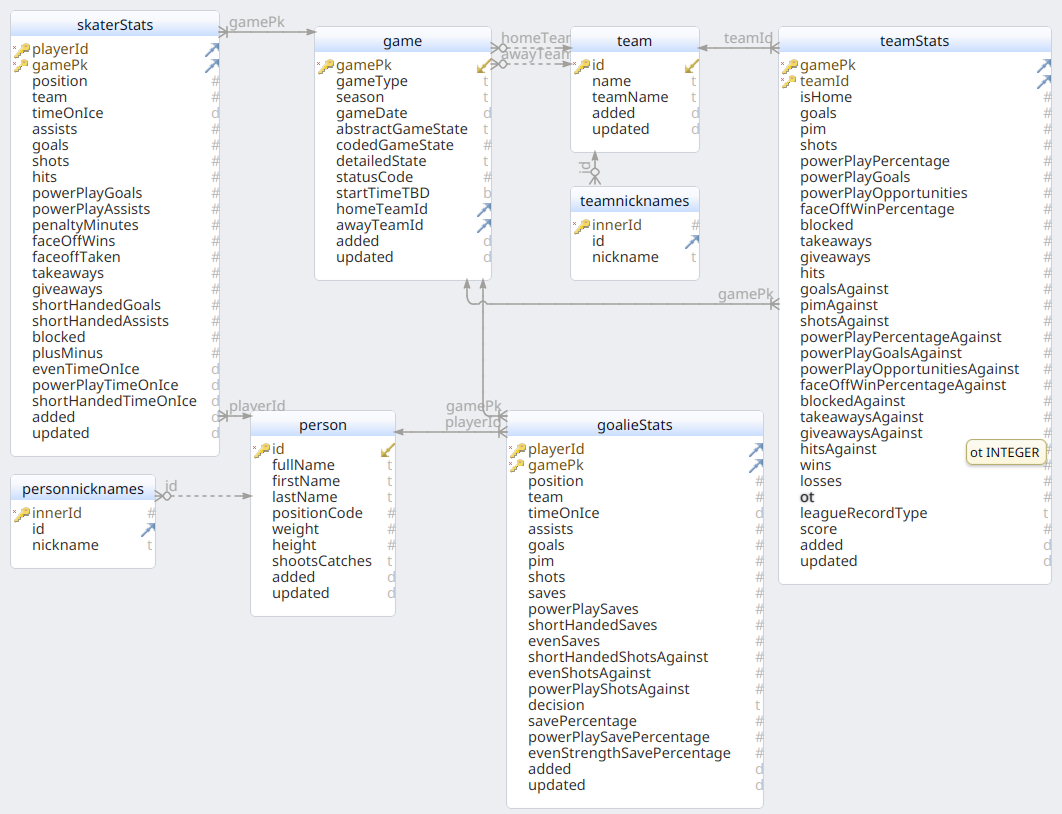
\includegraphics[width=\textwidth]{dbschema}
			\end{figure}
		
		\subsection{Data fetch from database}
			Thanks to storing data in database features was easy to shape and obtain with single SQL query:
\begin{minted}[xleftmargin=\parindent,linenos,breaklines]{sql}
SELECT person.id,person.positionCode,person.weight,person.height,person.shootsCatches,
skaterStats.timeOnIce,skaterStats.assists,skaterStats.goals,skaterStats.shots,
skaterStats.hits,skaterStats.powerPlayGoals,skaterStats.powerPlayAssists,
skaterStats.penaltyMinutes,skaterStats.faceOffWins,skaterStats.faceoffTaken,
skaterStats.takeaways,skaterStats.giveaways,skaterStats.shortHandedGoals,
skaterStats.shortHandedAssists,skaterStats.blocked,skaterStats.plusMinus,
skaterStats.evenTimeOnIce,skaterStats.powerPlayTimeOnIce,
skaterStats.shortHandedTimeOnIce FROM person,skaterStats WHERE person.positionCode != 'G' AND person.id = skaterStats.playerId
\end{minted}
			This SQL query performs join of players personal data like weight, height etc with players game statistics.
		
		\subsection{Data cleansing and transformation}
			Variables were classified into continuous variables and binary variables. This process is necessary to normalize \
			variables and convert binary variables to 0's or 1's there is only one binary variable person.shootsCatches which is information about dominant hand.
			
			Although four variables needed to be transformed shootsCatches and time statistics which were obtained as text and needed to be converted integer value. The example of time conversion from string to integer is presented below:
			
\begin{minted}[xleftmargin=\parindent,linenos,breaklines]{python}
nhl['timeOnIce'] = nhl['timeOnIce'].str.split('.').str[0]
nhl['timeOnIce'] = nhl['timeOnIce'].str.split(':').apply(lambda x: int(x[0]) * 60 + int(x[1]))
\end{minted}
			
			shootsCatches representing a dominant hand was converted using python pandas python library function factorize which transformed this variable to {0,1}:
			
\begin{minted}[xleftmargin=\parindent,linenos,breaklines]{python}
nhl.shootsCatches = pd.Categorical(pd.factorize(nhl.shootsCatches)[0])
\end{minted}
			
	\subsection{Data normalization}
	Data was normalized prior to using Linear Support Vector Classification, by using standard scaler which scales data to range of [0,1]. This is important because SVC tries to maximize the distance between the separating plane and the support vectors. If one feature (i.e. one dimension in this space) has very large values, it will dominate the other features when calculating the distance. If data is rescaled all features have the same influence on the distance metric. This was done by making a pipeline with standard scaler and SVC classifier. 
	
	 \begin{figure}[H]
        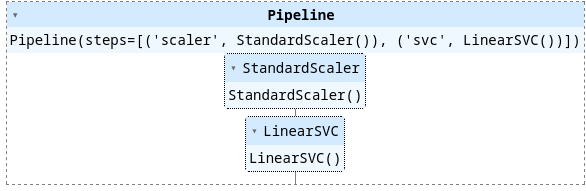
\includegraphics[width=\textwidth]{pipeline}
    \end{figure}
			
	\subsection{Testing data}
	Variance Threshold is a feature selector that removes all the low variance features from the dataset that are of no great use in modeling. It looks only at the features, not the desired outputs, and can thus be used for unsupervised learning. In other words it's used to find constant/quasi-constant predictors.
	
\begin{minted}[xleftmargin=\parindent,linenos,breaklines]{python}
from sklearn.feature_selection import VarianceThreshold
selector = VarianceThreshold()
selector.fit_transform(kb_features)
selector.get_feature_names_out()

array(['id', 'weight', 'height', 'shootsCatches', 'timeOnIce', 'assists',
       'goals', 'shots', 'hits', 'powerPlayGoals', 'powerPlayAssists',
       'penaltyMinutes', 'faceOffWins', 'faceoffTaken', 'takeaways',
       'giveaways', 'shortHandedGoals', 'shortHandedAssists', 'blocked',
       'plusMinus', 'evenTimeOnIce', 'powerPlayTimeOnIce',
       'shortHandedTimeOnIce'], dtype=object)
\end{minted}
	From the output of Variance Threshold it can be seen that there is no static or quasi-static predictors and all of the data is equally important.
	
	\subsection{Data split}
	Before attempting to use SVC data was splitted into train and test sets. With 75\% of data being set as train data and 25\% as test data.
\begin{minted}[xleftmargin=\parindent,linenos,breaklines]{python}
X_train, X_test, Y_train, Y_test = train_test_split(features, targets, test_size=0.25,random_state=0,shuffle=True)
\end{minted}
	
	\section{Method}
	After preparing the data linear SVC was used on training set to prepare fit coefficients that would be then used on test set.
\begin{minted}[xleftmargin=\parindent,linenos,breaklines]{python}
import warnings
warnings.filterwarnings("ignore")
from sklearn.model_selection import cross_val_score
from sklearn.tree import DecisionTreeClassifier
from sklearn.model_selection import train_test_split
from sklearn.svm import LinearSVC
from sklearn.pipeline import Pipeline
from sklearn.preprocessing import StandardScaler

pipe = Pipeline([('scaler', StandardScaler()), ('svc', LinearSVC())])
pipe.fit(X_train, Y_train)
print("Accuracy {:.2f}%".format(pipe.score(X_test, Y_test)*100))
\end{minted}

Which gave the accuracy of 73.52\%
\chapter{Results and Discussion}
	\section{Results}
	Even with not bad accuracy of 73.52\% at first attempt it was worth to check confusion matrix to target low accuracy classification results.
	
	\begin{figure}[H]
        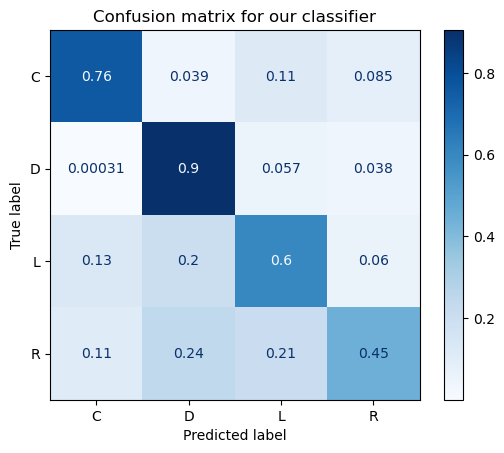
\includegraphics[width=0.6\textwidth]{matrix}
    \end{figure}
	
	\begin{itemize}
		\item the highest accuracy is for defence (D) players it's 90\% there would probably be not much space for optimization here
		\item center position (C) has 76\% accuracy it can be optimized a little to achieve better accuracy
		\item the two worst cases are left wing (L) and right wing (R) players for whom accuracy is 60\% and 45\%
	\end{itemize}
	
	\section{Discussion}
	\begin{itemize}
		\item what stands opposite to domain knowledge is that there is about 20\% probability of classifying wing players as defence players, stats of players from one line should be similar and thus probability of false positives should appear between those positions
		\item it's worth checking whether model could be optimized by dropping some of the player data from training set, especially the ones that for example have time on ice lower then average of other players at that position
		\item from the model it follows that defence players statistics vary significantly from centre and wing players thus accuracy for defence is very high
		
	\end{itemize} 
 

	
\chapter{Conclusion and References}
	\section{Conclusion}
		\begin{itemize}
			\item Sophisticated model would help NHL teams to figure out which players they should acquire and sell to keep necessary backup for line positions,
			\item NHL teams could use this model to figure out which players should play on which position to unleash their true potential based on statistics,
			\item According to Variance Treshold all of the columns are important for position classification,
			\item Defence position classification is almost certainly true,
		\end{itemize}
	\section{References}
		\begin{itemize}
			\item Matsuzawa, Takehiro. 2017. Using Machine Learning to Predict Future Points in the NHL
			\item Matt Eland, Predicting Hockey Penalties with Azure Machine Learning
		\end{itemize}
\end{document}
 
